\documentclass[a4paper,12pt]{article}
\usepackage{polyglossia}
\setdefaultlanguage{czech}

\usepackage{fontspec}
\usepackage{xunicode}

\usepackage{xltxtra}
\usepackage{tabularx}

\usepackage{makeidx}
\makeindex

% živé odkazy v PDF
\usepackage{hyperref}
\hypersetup{colorlinks=true, linkcolor=tul, urlcolor=tul, citecolor=tul}
\hypersetup{pdftitle={Semestrální práce}}
\usepackage[FM,fonts,noheader]{tul}
\usepackage{amsmath}
\usepackage{pdfpages}

\TULmail{daniel.adamek@tul.cz}
% definice příkazů a prostředí specifických pro tento dokument
\newcommand{\cmdfont}[1]{\texttt{\color{\tulcolor}#1}}
\newcommand{\cmdnoindex}[1]{\cmdfont{\textbackslash #1}}
\newcommand{\cmd}[1]{\cmdnoindex{#1}\index{#1@\textbackslash #1}}
\newcommand{\demobox}{\raisebox{-.20ex}{\rule{1em}{1em}}}
\newenvironment{itemize*}%
{\begin{itemize}%
     \setlength{\parskip}{0.25\baselineskip}%
     \setlength{\itemsep}{0pt}%
     \setlength{\partopsep}{0pt}%
     \setlength{\topsep}{0pt}}%
     {\end{itemize}}


\parindent=0pt
\parskip=0.5\baselineskip
\sloppy

\newcommand{\cmddemo}[1]{\bigskip\parbox[c]{3.9cm}{\cmd{#1}}\parbox[c]{10cm}{\csname #1\endcsname}\bigskip}

\begin{document}
\TULtitlepage{Dokumentace semestrální práce z předmětu ALG1}{Daniel Adámek}{Liberec 2022}

\section{Požadavky}
     \subsection{Zadání}
          Napište program, který načte dvě čtvercové matice stejné velikosti
          a zjistí, zda-li druhá matice vznikne jednoduchou \textit{(rotací)}
          o 0, 90, 180 nebo 270 stupňů v pravotočivém směru.
     \subsection{Specifikace vstupu}
          Program má umožnit při jednom spuštění zpracování libovolného počtu zadání. Pro každou úlohu program dostane od uživatele celé číslo jako rozměr
          zpracovávaných matic, poté budou načítány jednotlivá čísla matice (po řádcích). Pro každé zadání nechť program vypíše informaci, zda druhá ze zadaných matic vznikne
          z první některou z uvedených transformací.

          Program nechť výsledek svého šetření vypisuje jako jednu z následujících krátkých textových zpráv:
          \begin{itemize*}
               \item „Rotace 0“,
               \item „Rotace 90“,
               \item „Rotace 180“,
               \item „Rotace 270“,
               \item „Není rotace“.
          \end{itemize*}

          Po načtení záporného nebo nulového čísla místo rozměru matice nechť program skončí svoji činnost.

          \textbf{Poznámka}: pro dvě zadané matice může být nalezeno i více transformací.

          Program předpokládá, že:
          \begin{itemize*}
               \item všechny vstupní hodnoty zadané od uživatele budou právě typu integer,
               \item počet vstupních hodnot do matice bude roven počtu prvků matice, tj. druhá mocnina jednoho z jejích rozměrů.
          \end{itemize*}
\newpage
\section{Návrh řešení}
     Řešení spočívá v:
     \begin{itemize}
          \item načtení velikosti matic a tím inicializace třídy Matrix reprezentující matici;
          \item načtení obsahu obou matic;
          \item otáčení matic od 0 stupňů po 270 s krokem 90 stupňů;
          \item je-li matice jedním z možných otočení, program vypíše "Rotace " a počet stupňů;
          \item v případě, že druhá matice není žádnou možnou rotací matice první, program vypíše "Není rotace";
          \item program končí, pokud je zadaná velikost matice menší, nebo rovna nule.
     \end{itemize}
     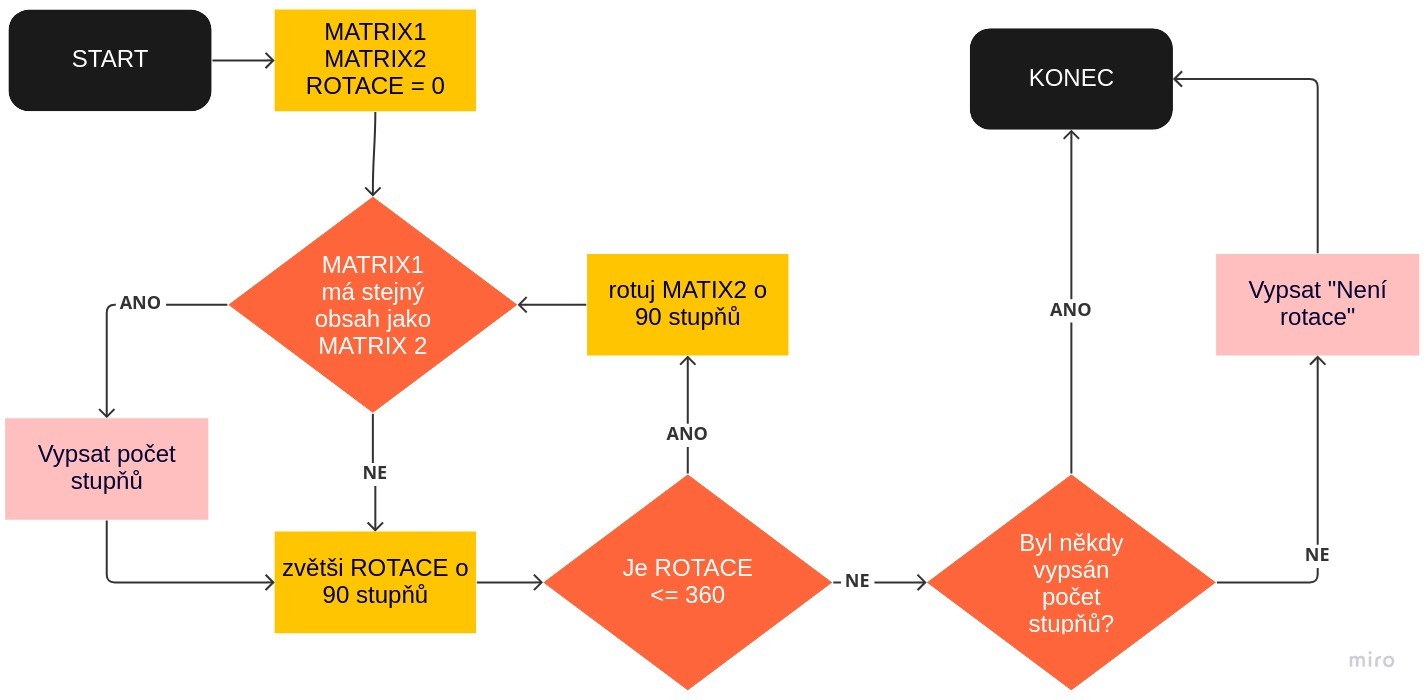
\includegraphics[scale=0.36]{alg1-flowchart}

     Samotné otočení matice spočívá v:
     \begin{itemize}
          \item převrácení řádků v matici;
          \item tranpozice matice.
     \end{itemize}

     
\includegraphics[scale=0.18]{alg1-rotate-flowchart}

\section{Protokol o testování}
     K testování jsem použil nástroj JUnit5, její metody \textit{assertTrue, assertNotSame} a třídu MatrixTest.
     Při testování se v některých případech využívá náhodně generovaných čísel, pro zobecnění vstupů testů.
     Kompletní report generovaný přímo JUnit se nachází v souboru \textit{Test Results - MatrixText.pdf} v repozitáři
     společně s touto zprávou. Níže vypsaná tabulka je přimá interprezace dat ze zmiňovaného PDF souboru.

\subsection{Záznam o testování}

     \textbf{Číslo testu:} 1\\
     \textbf{Typ testu, popis vstupů:} Test metody hasSameContent() třídy Matrix s náhodnými hodnotami od -1000 do 1000;
     metoda prochází každý element 2 dimenzionálního pole dat třídy Matrix a hodnotí, zda-li mají matice stejný obsah.\\
     \textbf{Doba testu:} 1ms \\
     \textbf{Očekávaný výsledek:} Správné zachycení situace, kdy matice při inicializaci je vyplněná nulami a zároveň
     na pozici s indexem 1-1 je manuálně nastavena hodnota 1 a neodpovídá
     matici, která má náhodně vygenerované hodnoty od -1000 do 1000 a zároveň na pozici s indexem 1-1 je manuálně
     nastavena hodnota 2; dále při manuálním kopírování pomocí for-cyklů je obsah obou matic identický.\\
     \textbf{Skutečný výsledek:} Matice náhodně vygenerovaná a nulová matice s 1 prvkem nenulovým jsou identifikovány
     jako jiné a zároveň matice manuálně kopírované jsou vyhodnoceny jako mající stejné hodnoty.\\
     \textbf{Prošel (ANO/NE):} ANO\\

     \textbf{Číslo testu:} 2\\
     \textbf{Typ testu, popis vstupů:} Test metody deepCopy() třídy Matrix s náhodnými hodnotami od -1000 do 1000;
     metoda na vytváří nový objekt třídy Matrix se stejným obsahem a jinou referencí (hluboká kopie).\\
     \textbf{Doba testu:} 1ms\\
     \textbf{Očekávaný výsledek:} Správné vytvoření třídy, provedení hluboké kopie pomocí metody deepCopy(); očekává se průchod testy porovnání referencí pole dat objektu a porovnání jeho obsahu.\\
     \textbf{Skutečný výsledek:} Reference na pole dat objektů nejsou stejné $\implies$ jsou to jiné objekty a obsah je totožný - ověření pomocí metody hasSameContent\\
     \textbf{Prošel (ANO/NE):} ANO\\

     \textbf{Číslo testu:} 3\\
     \textbf{Typ testu, popis vstupů:} Manuální rotace matice 2x2 o obsahu
          \[\begin{pmatrix}
               1 & 2 \\
               3 & 4
          \end{pmatrix}\] po otočení o 90 stupňů v definovaném směru dle zadání má tvar\\
          \[\begin{pmatrix}
                    3 & 1\\
                    4 & 2
          \end{pmatrix}\]
     \textbf{Doba testu: 16ms \textit{(kvůli inicializaci JUnit)}} \\
     \textbf{Očekávaný výsledek:} Úspěch porovnání otočené matice pomocí metory turn() a manuálně otočené matice\\
     \textbf{Skutečný výsledek:} Matice otočená o 90 stupňů pomocí metody je ta samá jako otočená manuálně.\\
     \textbf{Prošel (ANO/NE):} ANO\\

     \textbf{Číslo testu:} 4\\
     \textbf{Typ testu, popis vstupů:} Test otáčení - mezní hodnoty; zkouší se matice o rozměru strany 0 a 1
     \textbf{Doba testu:} 1ms \\
     \textbf{Očekávaný výsledek:} Úspěch porovnání stejného obsahu u matice otočené matice pomocí metody turn()
     o 90 stupňů a poté o 180 a matice a otočené matice o 180 stupňů a poté o 90 a další otáčení.\\
     \textbf{Skutečný výsledek:} Všechna otočení proběhla korektně.\\
     \textbf{Prošel (ANO/NE):} ANO\\

     \textbf{Číslo testu:} 5\\
     \textbf{Typ testu, popis vstupů:} Test otáčení - liché velikosti matic; zkouší se matice o lichém rozměru strany
     \textbf{Doba testu:} 4ms \\
     \textbf{Očekávaný výsledek:} Úspěch porovnání stejného obsahu u matice otočené matice pomocí metody turn()
     o 90 stupňů a poté o 180 a matice a otočené matice o 180 stupňů a poté o 90 a další otáčení.\\
     \textbf{Skutečný výsledek:} Všechna otočení proběhla korektně.\\
     \textbf{Prošel (ANO/NE):} ANO\\

     \textbf{Číslo testu:} 6\\
     \textbf{Typ testu, popis vstupů:} Test otáčení - sudé velikosti matic; zkouší se matice o sudém rozměru strany
     \textbf{Doba testu:} 4ms \\
     \textbf{Očekávaný výsledek:} Úspěch porovnání stejného obsahu u matice otočené matice pomocí metody turn()
     o 90 stupňů a poté o 180 a matice a otočené matice o 180 stupňů a poté o 90 a další otáčení.\\
     \textbf{Skutečný výsledek:} Všechna otočení proběhla korektně.\\
     \textbf{Prošel (ANO/NE):} ANO\\
\section{Fotodokumentace výsledků testů}
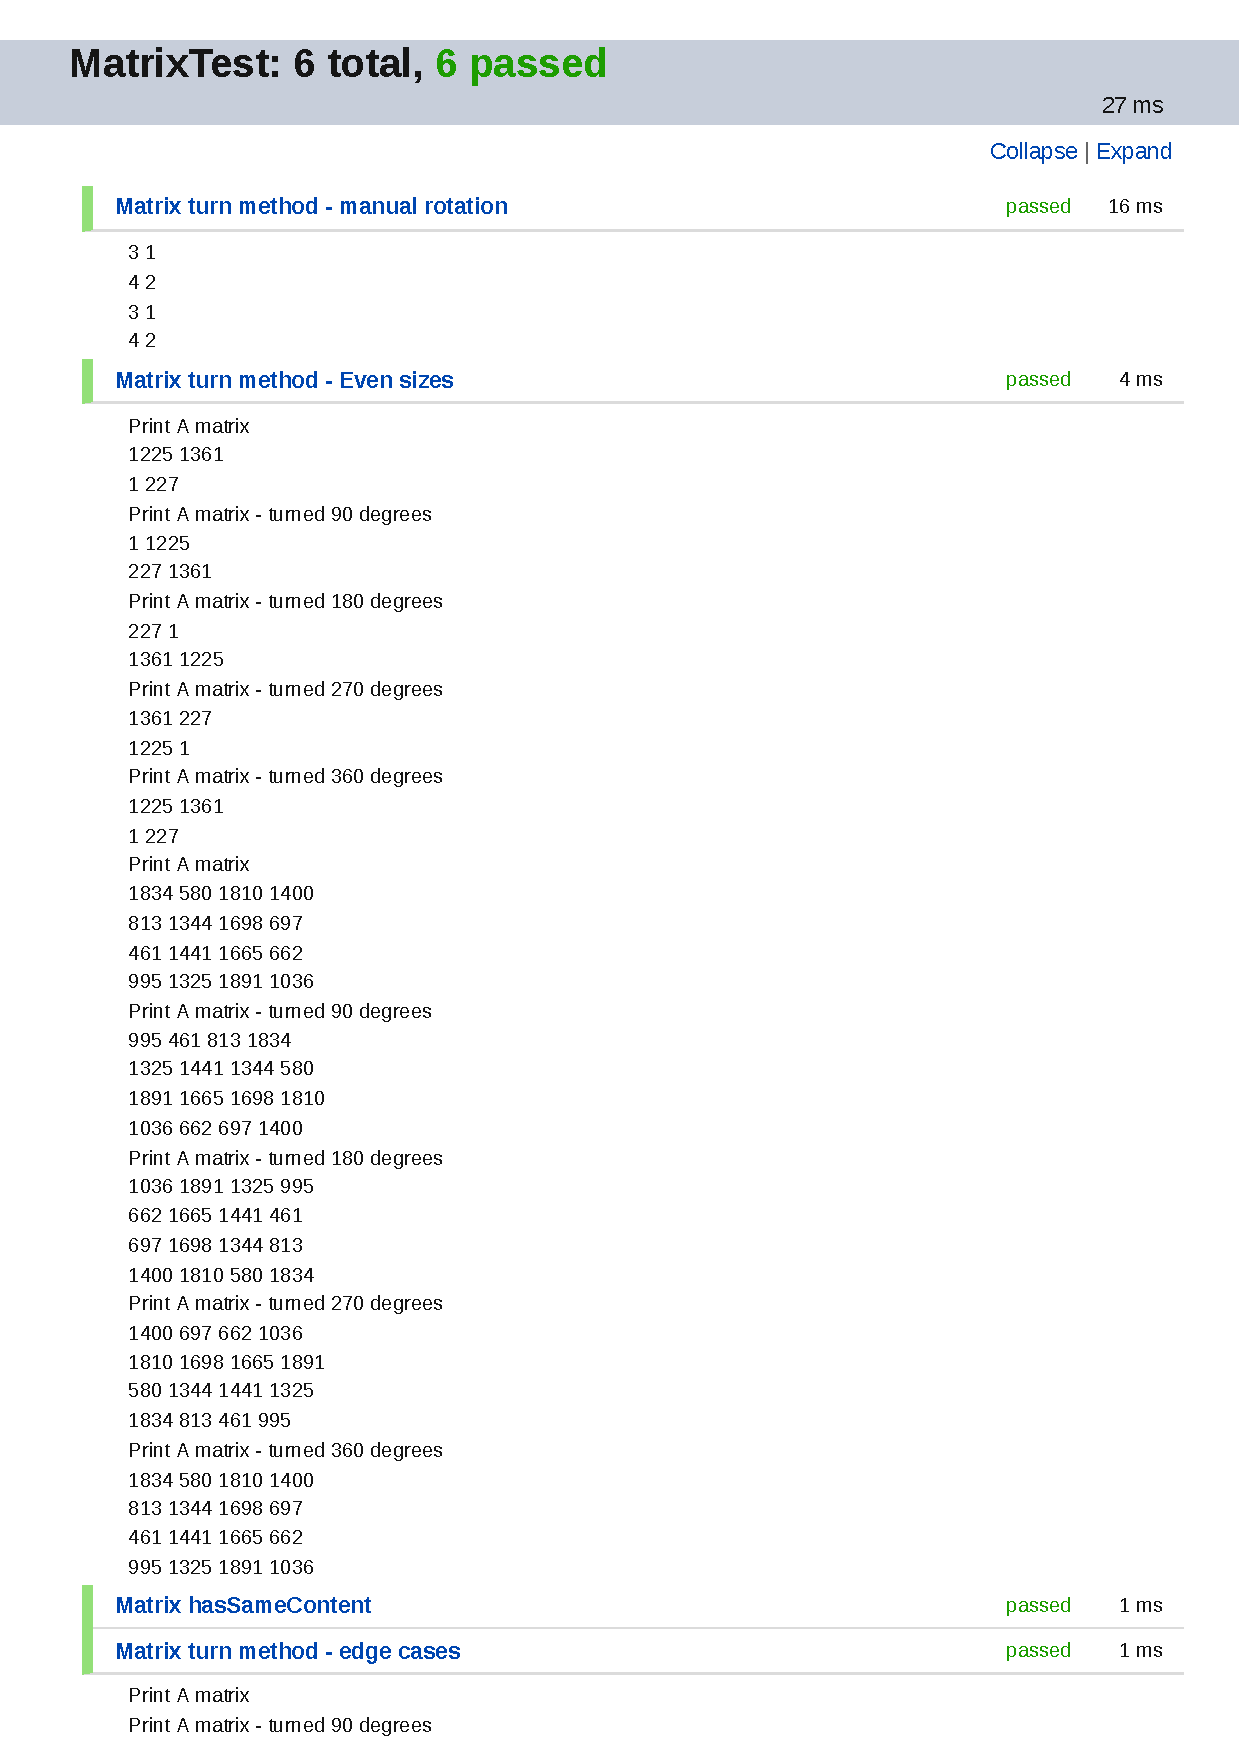
\includepdf[pages=-]{Test Results - MatrixTest.pdf}

\end{document}
